Cette annexe utilise le logiciel LARP qui est gratuit depuis le 1\textsuperscript{er} Mars 2008, téléchargeable à l'adresse suivante \url{http://www.larp.marcolavoie.ca/fr/default.htm}, et qui malheureusement ne fonctionne que sous Windows\textsuperscript{\textcopyright}. 
LARP, qui est l'acronyme de Logiciel d'Algorithmes et de Résolution de Problèmes, permet au choix de taper des programmes ou bien d'utiliser des algorigrammes.
La seconde option permet de produire l'algorigramme ci-dessous qui propose une méthode de résolution dans $\RR$ d'une équation polynomiale du second degré
\footnote{
	Nul besoin de connaître cette théorie qui est généralement abordée en classe de première. L'idée ici est juste de comparer \og visuellement \fg{} différentes représentations d'un algorithme non simplistes.
}
où nous supposons implicitement que $a \neq  0$.

\begin{center}
	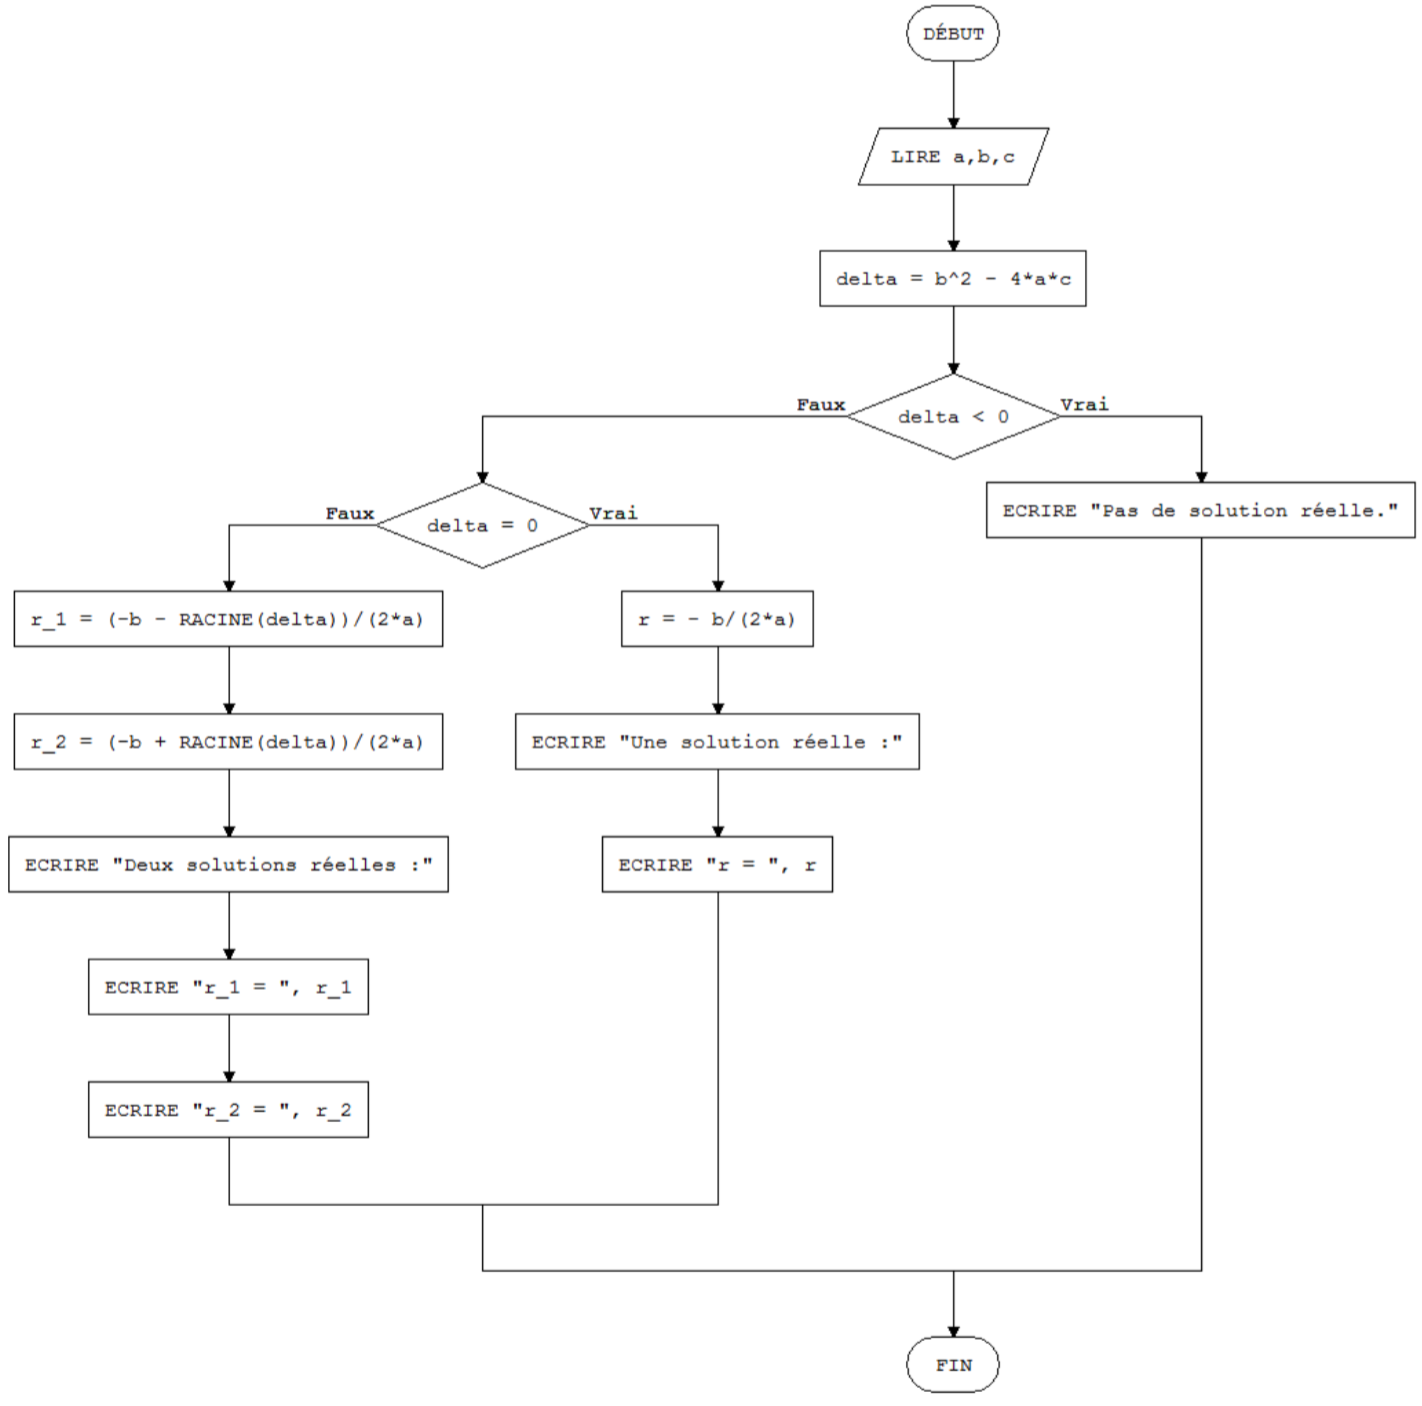
\includegraphics[width=1\textwidth]{reading/draw_limits/real_quadratic_equations.png}
\end{center}


LARP permet de produire directement une version \og programme \fg{} de l'algorigramme précédent. Nous obtenons ce qui suit où de nouveau nous supposons implicitement que $a \neq  0$.

\newpage

\begin{myverb}
DÉBUT
    LIRE a,b,c
    delta = b^2 - 4*a*c
    SI delta < 0 ALORS
        ECRIRE "Pas de solution réelle."
    SINON
        SI delta = 0 ALORS
            r = - b/(2*a)
            ECRIRE "Une solution réelle :"
            ECRIRE "r = ", r
        SINON
            r_1 = (-b - RACINE(delta))/(2*a)
            r_2 = (-b + RACINE(delta))/(2*a)
            ECRIRE "Deux solutions réelles :"
            ECRIRE "r_1 = ", r_1
            ECRIRE "r_2 = ", r_2
        FINSI
    FINSI
FIN

\end{myverb}
\bigskip

La comparaison des deux représentations précédentes montre qu'un algorigramme devient vite très encombrant. La version symbolique ci-après montre que l'on peut faire encore mieux.


\bigskip
\begin{algo}
    \Data{$(a , b , c) \in \RR^3$ où l'on suppose $a \neq  0$}
    \Begin{
	$\Delta = b^2 - 4 ac$ \\
        \eIf{$\Delta < 0$}{
		\Print{"Pas de solution réelle."}
        }{
		\eIf{$\Delta = 0$}{
			$r = \dfrac{-b}{2a}$ \\
			\vspace{0.5em}
			\Print{"Une solution réelle :"} \\
			\Print{"r = ", r} \\
        	}{
			$r_1 = \dfrac{-b - \sqrt{\Delta}}{2a}$
			et
			$r_2 = \dfrac{-b + \sqrt{\Delta}}{2a}$ \\
			\vspace{0.5em}
			\Print{"Deux solutions réelles :"} \\
			\Print{"$r_1$ = ", $r_1$} \\
			\Print{"$r_2$ = ", $r_2$} \\
		}
	}
    }
\end{algo}
\bigskip


En résumé, les algorigrammes sont un très bon outil quand l'on prend contact avec les algorithmes et la programmation mais ils montrent très vite leur limite quand on s'attaque à de \og vrais \fg{} problèmes.